\section{Theoretical Analysis}
\label{sec:analysis}

In this section, the circuit shown in \textbf{Figure~\ref{fig:diagram_t2}} is analysed
theoretically.\par

\begin{figure}[h!] \centering
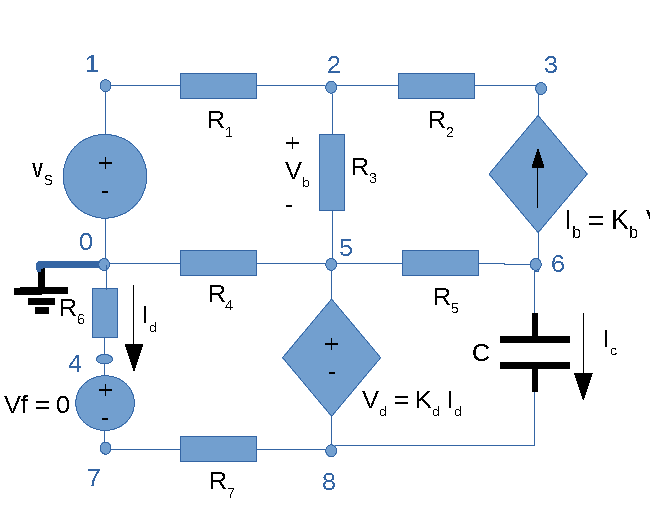
\includegraphics[width=0.6\linewidth]{diagram_t2.pdf}
\caption{Diagram of the circuit considered for the computations and simulations}
\label{fig:diagram_t2}
\end{figure}

%point 1
\subsection{Analysis for $t<0$} 
The nodal method is aplied to the circuit in order to determine the voltage in all nodes and the current on all branches . The nodal method aplies KVL and for $t<0$ no current passes through the capacitor, and therefore this component behaves like an open circuit.
%In \textbf{Table~\ref{tab:theoretical}} the values for the branch currents and the node voltages obtained from the Octave script for both methods are presented. Here, the node voltages in the mesh method were computed from the respective currents, which were determined as described in the previous subsection.
 
\begin{table}[h!]
  \centering 
  \begin{tabular}{|l|r|}
    \hline    
    {\bf Name} & {\bf Node method}\\ \hline
    V0 & 0\\ \hline
V1 &  5.054818641360000\\ \hline
V2 &  4.793704691824189\\ \hline
V3 &  4.258197784082119\\ \hline
V4 & -1.934225550007436\\ \hline
V5 &  4.831047093349573\\ \hline
V6 &  5.668298372306746\\ \hline
V7 & -1.934225550007436\\ \hline
V8 & -2.905231322705667\\ \hline
Ir1 &   -2.536487650531725e-01\\ \hline
Ir2 &   -2.658975828505401e-01\\ \hline
Ir3 &    1.224881779736725e-02\\ \hline
Ir4 &  1.205310280142027\\ \hline
Ir5 &    2.658975828505403e-01\\ \hline
Ir6 &   -9.516615150888543e-01\\ \hline
Ir7 &   -9.516615150888547e-01\\ \hline
Gbn &    2.658975828505403e-01\\ \hline

  \end{tabular}
  \caption{A variable that starts with "Ir" and the variable "Gb" are of type {\em current}
    and expressed in milliampere (mA); all the other variables that start with a "V" are of the type {\it voltage} and expressed in
    Volt (V).}
  \label{tab:theoretical}
\end{table}

%point 2
\subsection{Equivalent resistor as seen from the capacitor terminals}

To compute the equivalent resistance as seen by C the independent source $V_c$ needs to be switched off. We do this by replacing it with a short circuit ($V_s=0$). We also replace the capacitor with a voltage source $V_x=V_6-V_8$.We use the $V_6$ and $V_8$ from the previous section beacause the voltage drop at the ends of the capacitor needs to be a continuous function (there can not be an energy spike in the capacitor). With this in mind a nodal analysis is performed in order to determine the current $I_x$ that is supplied by $V_x$.With this values we can determine $R_{eq}$ ($R_{eq}=V_x/I_x$). All this procedures were required in order to determine the time constant $\tau$ ($\tau=R_{eq}*C$). The time constant in crucial to determine the natural and forced solutions for $V_6$, which will be done in the next subsections. 

%In \textbf{Table~\ref{tab:theoretical}} the values for the branch currents and the node voltages obtained from the Octave script for both methods are presented. Here, the node voltages in the mesh method were computed from the respective currents, which were determined as described in the previous subsection.
\begin{table}[h!]
  \centering
  \begin{tabular}{|l|r|}
    \hline    
    {\bf Name} & {\bf Values for aux circuit}\\ \hline
    @Gb & 0.00000000000\\ \hline
@r1 & 0\\ \hline
@r2 & 0\\ \hline
@r3 & 0\\ \hline
@r4 & 0\\ \hline
@r5 &   -2.828260531660058e-03\\ \hline
@r6 & 0\\ \hline
@r7 & 0\\ \hline
v(1) & 0.00000000000\\ \hline
v(2) & 0.00000000000\\ \hline
v(3) & 0.00000000000\\ \hline
v(4) & 0.00000000000\\ \hline
v(5) & 0.00000000000\\ \hline
v(6) & 8.83130397945\\ \hline
v(7) & 0.00000000000\\ \hline
v(8) & 0.00000000000\\ \hline
Ix & -0.00282826053\\ \hline
Vx & 8.83130397945\\ \hline
$Req_{}$ & -3.122521e+03\\ \hline
$\tau$ & -3.181599e-03\\ \hline
  \end{tabular}
  \caption{A variable that stars with a "V" is of type {\it voltage} and expressed in
    Volt (V).The variable $R_{eq}$ is expresses in Ohm and the variable $\tau$ is expressed in seconds }
  \label{tab:equivalent resistor}
\end{table}
\vspace{10cm}
\pagebreak

%point 3
\subsection{Natural solution for $V_6$}

The natural solution depends on initial charge (voltage) and on $R_{eq}$ and C and it is computed by removing all independent sources and applying KVL.In Octave to compute the Natural solution the general formula derived in the theoretical classes was used: $V_{6n}(t)=Ae^{\frac{-t}{\tau}}$. In this formula $\tau$ is the time constant determined in the previous section and  A is a constant that can be determined through the boundry conditions (when $t=0$, $A=V_x$)

\begin{figure}[H] \centering
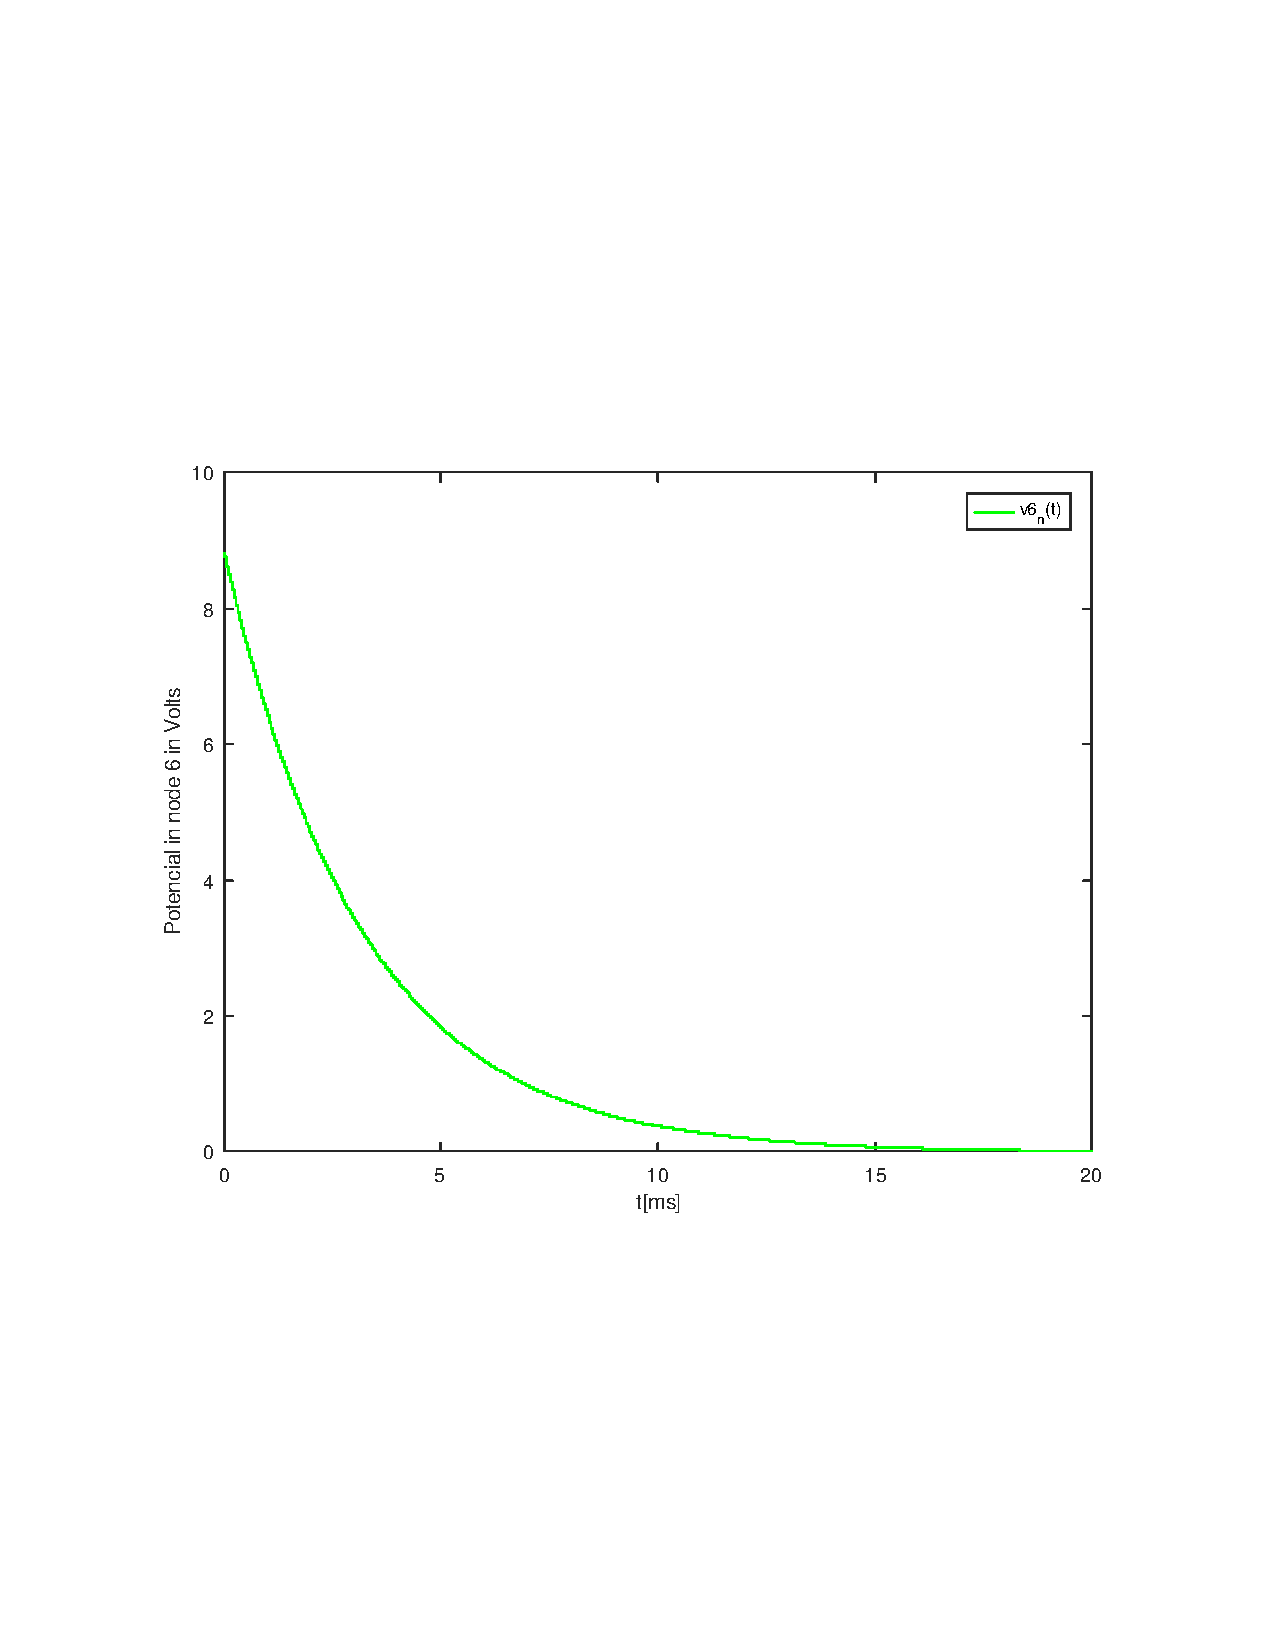
\includegraphics[width=0.9\linewidth]{natural_tab.pdf}
\caption{Natural response of $V_6$ as a function os time in the interval from [0,20] ms}
\label{fig:natural}
\end{figure} 

\pagebreak

%point 4
\subsection{Forced solution for $V_6$ with $f=1000Hz$}

In this section the forced solution $V_{6f}$ is determined for the same time interval and for a frequency of 1KHz. To do this a nodal analysis was used but insted of resistences and capacitances, impedences were used. It was also  considered that the magnitude of the phaser of the voltage sorce $V_s$  was 1 ($V_s=1$). By taking all these steps the phaser voltages in all nodes were determined. The complex amplitudes of the phasers are presented in  \textbf{Table ~\ref{tab:equivalent resistor}}
\begin{table}[h!]
  \centering
  \begin{tabular}{|l|r|}
    \hline    
    {\bf Name} & {\bf Complex amplitude voltage}\\ \hline
    V0 & 0\\ \hline
V1 &  1\\ \hline
V2 &    9.445310207903378e-01\\ \hline
V3 &    8.329148493139050e-01\\ \hline
V4 &    3.744381306846604e-01\\ \hline
V5 &    9.524211706387480e-01\\ \hline
V6 &    5.602948262043124e-01\\ \hline
V7 &    3.744381306846604e-01\\ \hline
V8 &    5.581602943867834e-01\\ \hline

  \end{tabular}
  \caption{Complex amplitudes in all nodes ***********quais são as unidades da amplitude V ou m?********}
  \label{tab:equivalent resistor}
\end{table}
\vspace{10cm}
\pagebreak

%point 5
\subsection{Final total solution $v_6(t)$}
In this section the final total solution $V_6$ for a frequency of 1KHz is determined by superimposing the natural and forced solutions determined in previous sections ($V_6$=$V_{n6}$+$V_{6f}$) In \textbf{Figure: ~\ref{fig:theo5}} the voltage of the independent font $V_{st}$ and the voltage of $V_{6}$ were ploted for the time interval of [-5,20] ms. 
\begin{figure}[h!] \centering
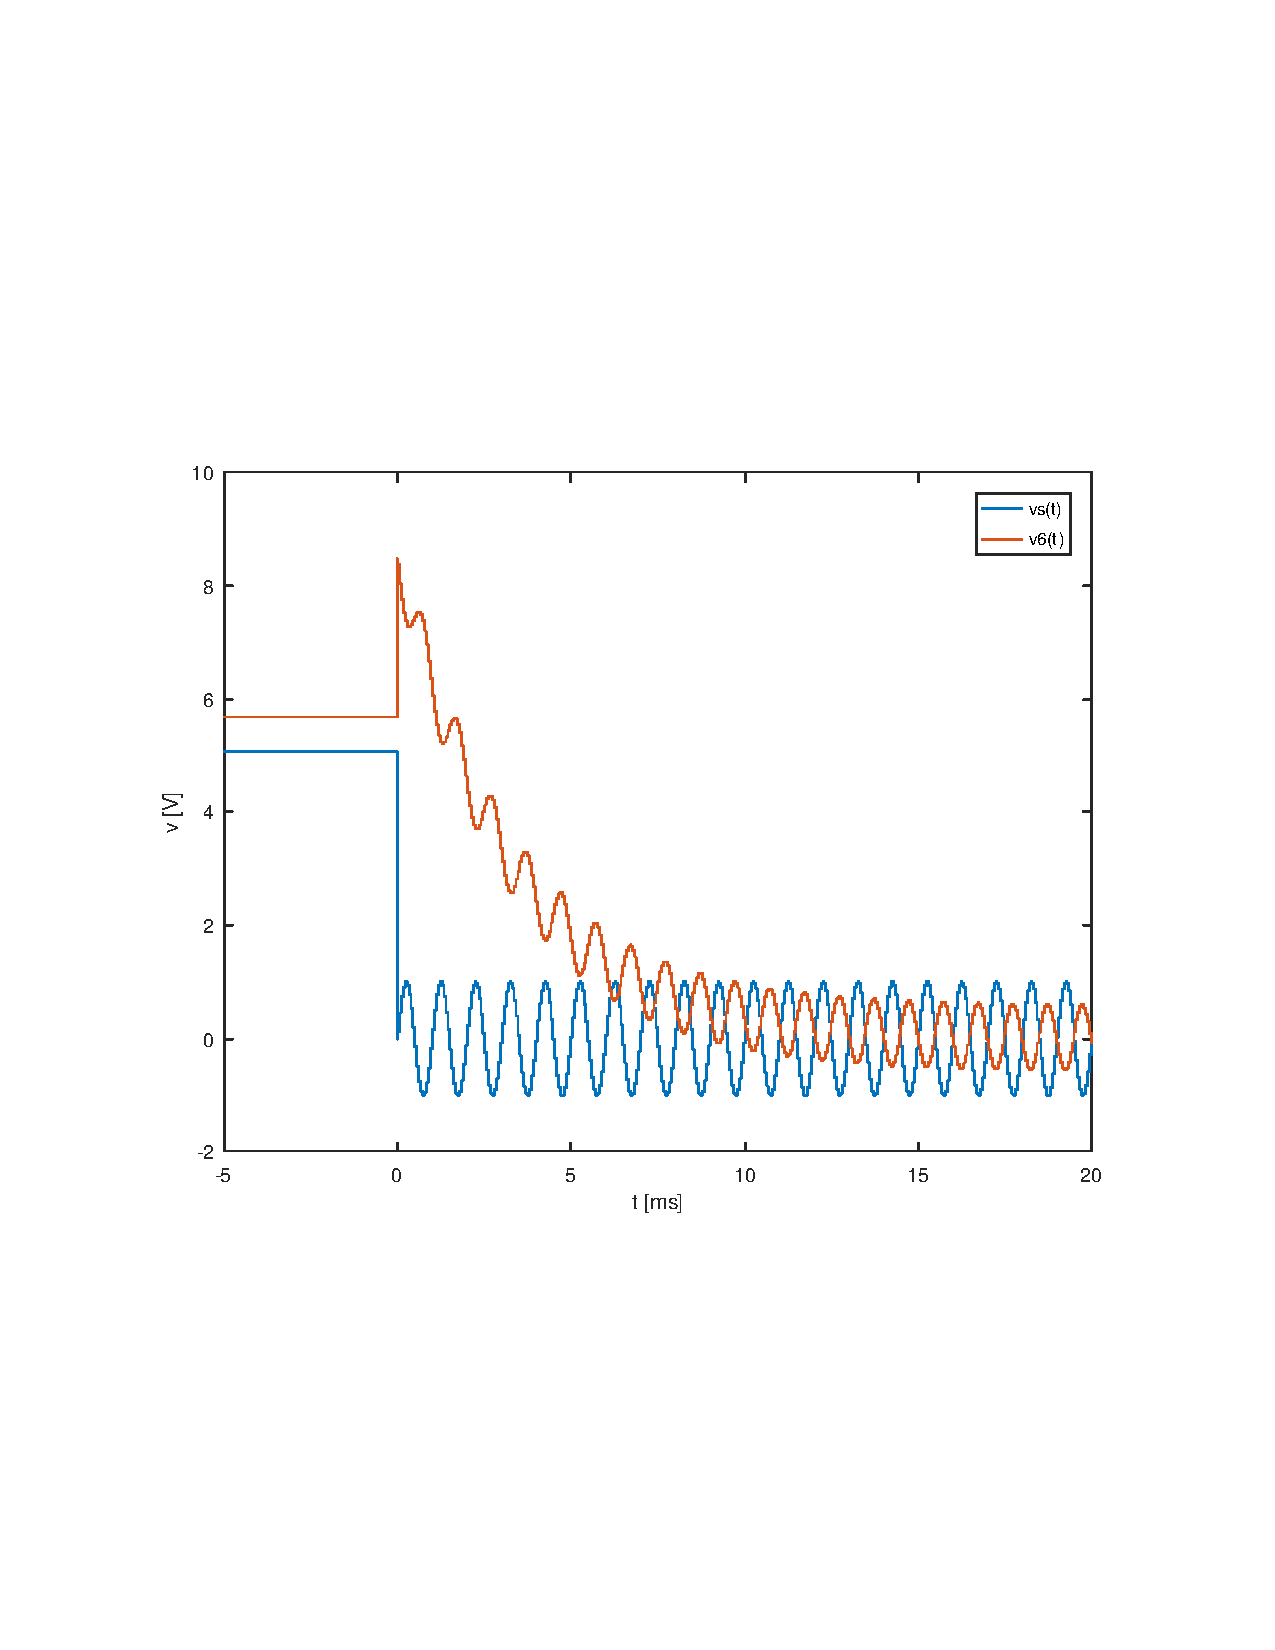
\includegraphics[width=0.9\linewidth]{theo5_tab.pdf}
\caption{Voltage of $V_{6}(t)$ and $V_{st}(t)$ as functions of time from [-5,20] ms}
\label{fig:theo5}
\end{figure}
\vspace{15cm}
\pagebreak


\subsection{Frequency responses $v_c(f)$, $v_s(f)$ and $v_6(f)$ for frequency range 0.1 Hz to 1 MHz}
\begin{figure}[h!] \centering
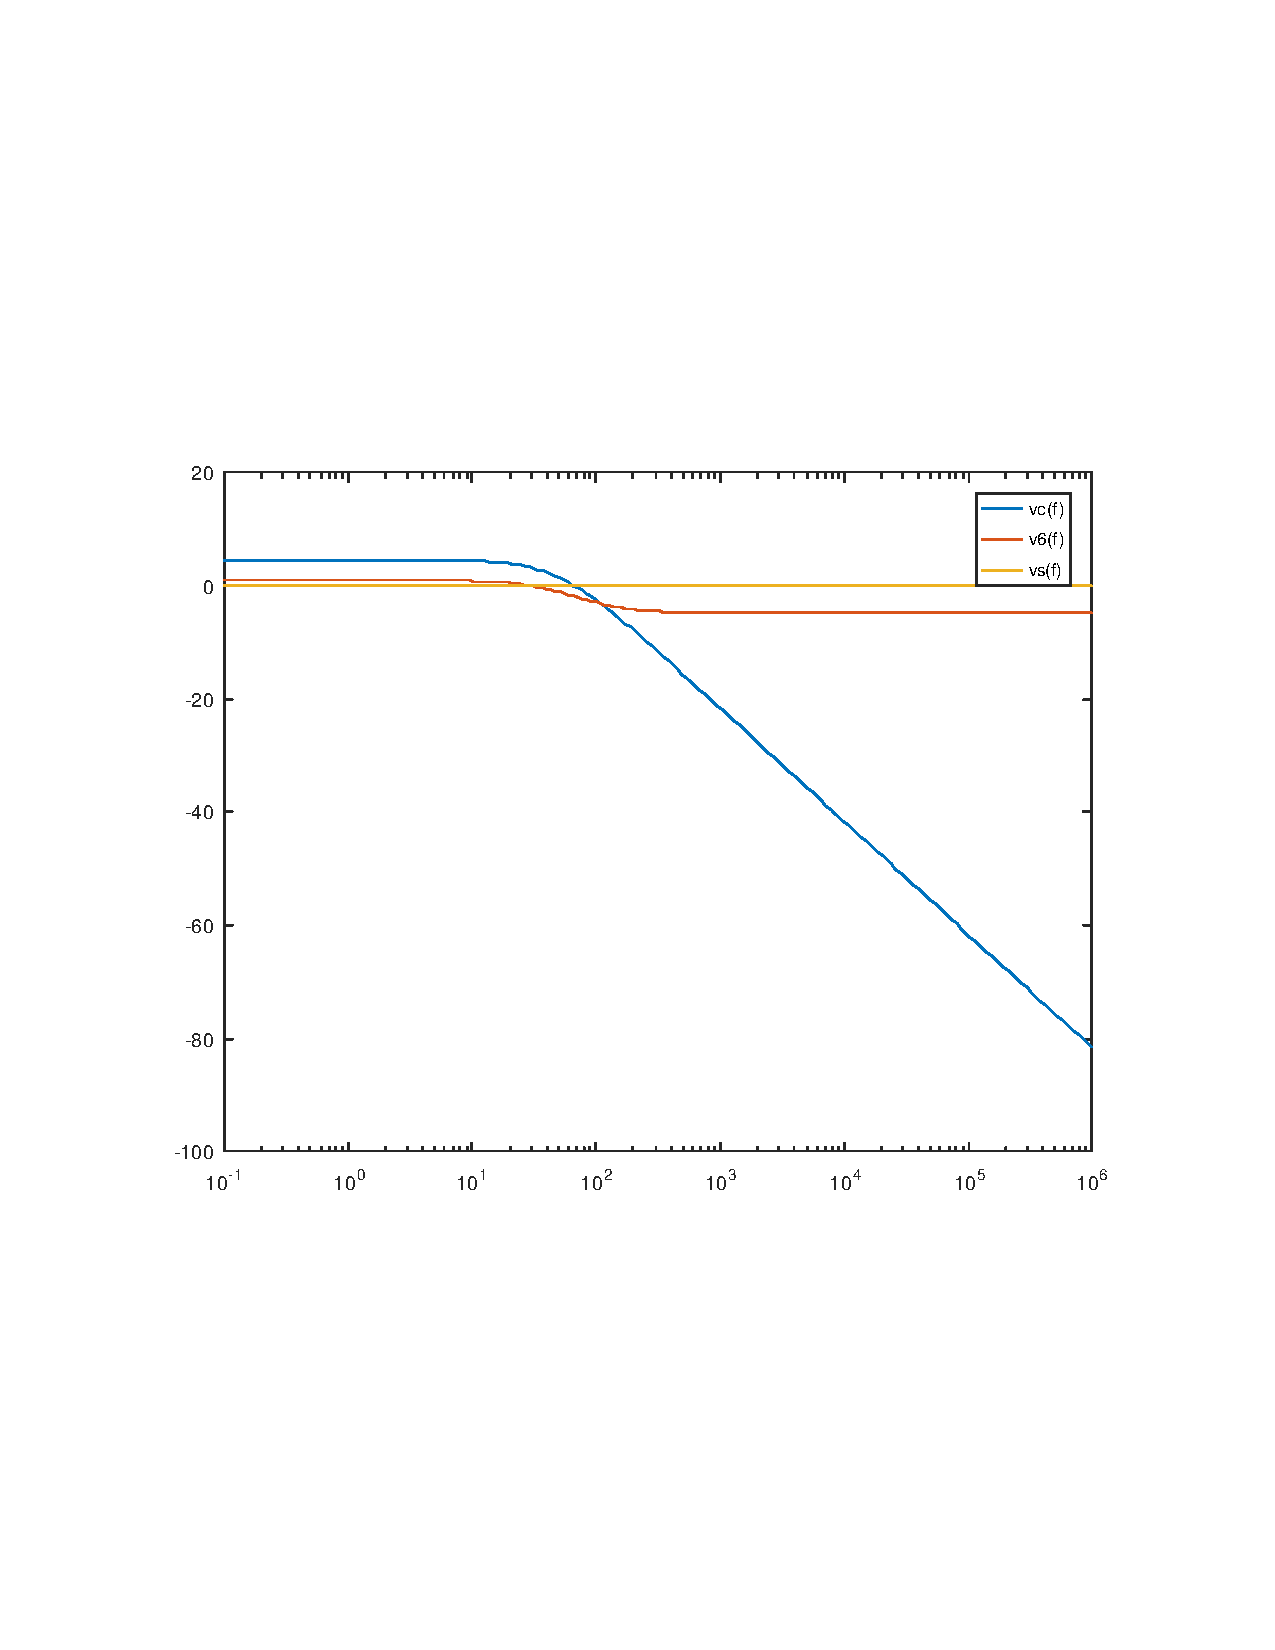
\includegraphics[width=0.9\linewidth]{freq_resp_tab.pdf}
\caption{point 6: Graph for amplitude frequency response of Vc, V6 and Vs for frequencies ranging from 0.1Hz to 1MHz}
\label{fig:freq_resp}
\end{figure}

\vspace{15cm}

\begin{figure}[h!] \centering
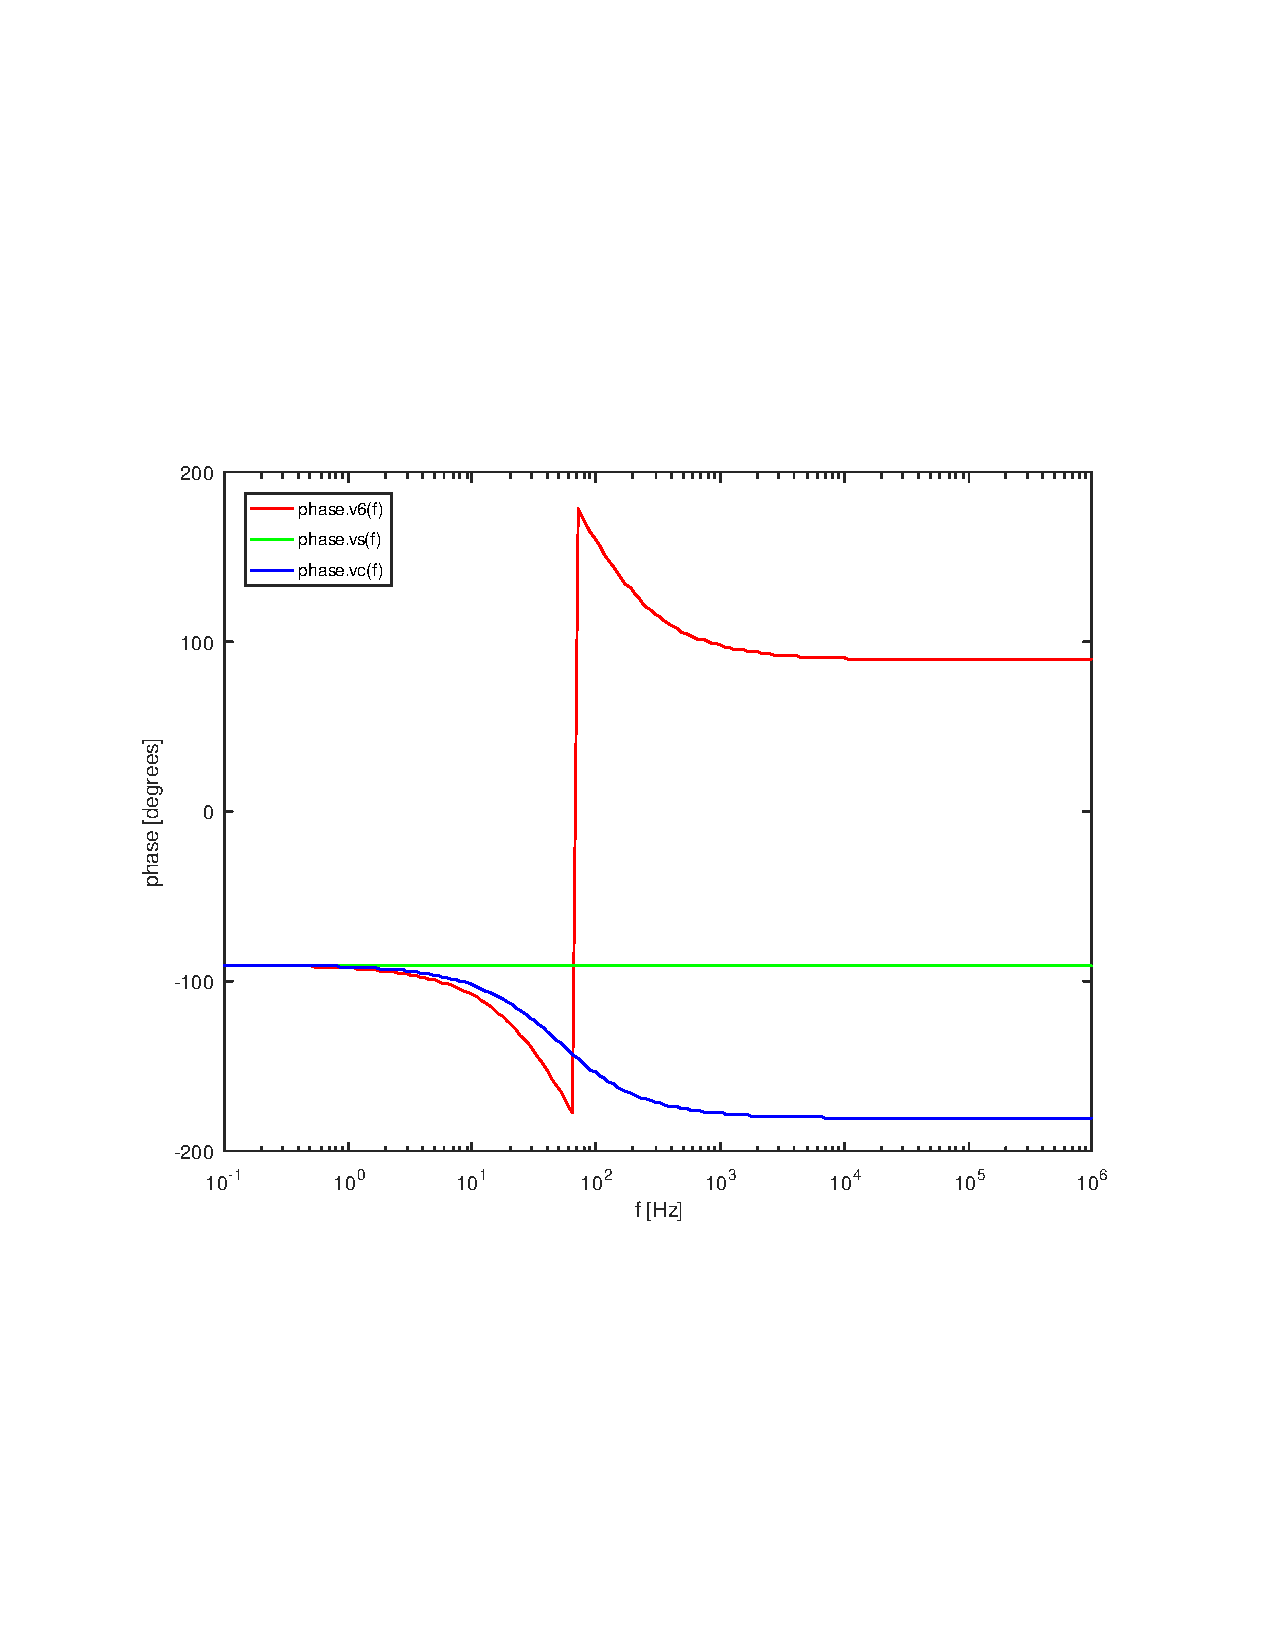
\includegraphics[width=0.9\linewidth]{angle_tab.pdf}
\caption{point 6: Graph for phase frequency response of Vc, V6 and Vs for frequencies ranging from 0.1Hz to 1MHz}
\label{fig:angle_resp}
\end{figure}

\vspace{15cm}



